%% Before beginning to type your dissertation, read the formatting guide, 
%% which can be found at http://grad.msu.edu/etd/docs/formattingguide.pdf
%% Also get the latest version of  msuphddissertation.cls and the template file
%% at http://www.math.msu.edu/~weil/MSU_Ph.D._Dissertation.zip
%% Send questions to weil@math.msu.edu
\documentclass{msuphddissertation}
\usepackage{amssymb, amsmath}
\usepackage{natbib}
%\usepackage{subcaption}
\usepackage{graphicx}
\usepackage{url}
%% Insert packages you wish to use except setspace and subfig. 
%% Those packages are loaded automatically.
%% IMPORTANT: Load only those packages you know you will use.
%% Some packages can cause conflicts resulting in improper formatting.
\author{Elijah K. Lowe} %% Put your name in full as it is officially recognized by Michigan State University here.
\title{The wood chipper problem: } %% Put the title of your dissertation here.
\unit{Computer Science \& Engineering} %% Put the name of your degree granting unit here. The complete
%% list of these degree granting units can be found at
%% http://grad.msu.edu/etd/docs/DegreeGrantingUnits.pdf

%% Put additional preamble items here.

%%%%%% LANDSCAPE PAGES  %%%%%%
%% The environment, landscapenum, produces a page in 
%% landscape mode and then rotates the page by 90 degrees 
%% making is readable on a computer screen, and places the page number
%% along the 11 inch side, which is the bottom of the rotated page. 

%%%%%%%%%%%%%%%%%%%%%%%%%%%%
%%%%%%%%  NOTE   %%%%%%%%%%%%%%
%% PREPARING A DISSERTATION WITH THIS CLASS FILE DOES NOT %%%
%% GUARANTEE THAT THE GRADUATE SCHOOL WILL APPROVE IT %%%
%%%%%%%%%%%%%%%%%%%%%%%%%%%%%%%

%%%%%%%%%%%%%%%%%%%%%%%%%%%%%%%%%%
%%%%%%%%%%%% WARNING %%%%%%%%%%%%%%%
%% The Graduate School requires that all text, except superscripts %%
%% and subscripts, but including text in imported %%
%% graphics files be in 12 point. For that reason it's recommended %%
%% that no text be part of any imported files. %%

%% Once your document has been filed with the Graduate School,
%% if you wish to produce a version of it whose subscripts and superscripts
%% are in traditional smaller proportion, remove the "%" sign 
%% in front of following command. 
%\DeclareMathSizes{12}{12}{10}{8}
%% If your document has footnotes, remove the "%" sign 
%% in front of following command. 
%\renewcommand{\footnotesize}{\small}
%% To single space your document, remove the 
%% two commands \begin{doublespace}
%% and \end{doublespace} below.

\begin{document}

\maketitlepage %%This command will produce the title page of your thesis.
\begin{abstract}
Abstract goes here
\end{abstract}

%% If you wish to have a copyright page, remove the "%" in front of  \begin{copyrt}
%% and remove the "%" in front of \end{copyrt}.
%% The mandatory form of the Copyright will be generated automatically. 
%% A copyright statement is optional.

%\begin{copyrt}
%\end{copyrt}
%% If you wish to have a dedication, remove the "%" in front of
%% \begin{dedication}
%% \end{dedication}
%% A dedication must be single-spaced and 
%% centered on the page.  Both will be done automatically. 

\begin{dedication}
\begin{center} 

\end{center}
\end{dedication}

%% If you wish to have an acknowledgment, remove the "%" in front of  \begin{acknowledgment}
%% and remove the "%" in front of  \end{acknowledgment}  
\begin{acknowledgment}
Where do I begin? I am a summation of all the people that I have come in contact throughout my life. So, I would like to dedicate this text to some of the most influential people. 

I start with my mother Patricia Lowe who always encouraged me to pursue my wildest dreams. My father William Robertson, who thought me to question the world and to always pay attention to the small things. My brother Fard Lowe, who consistently served as an inspiration to me and someone I could count on. To my high school consoler, Kathy Giles-Harris and high school math teacher, Christopher Reese who both saw something special in me, and pushed me to pursue it. 

My brothers from Morehouse\textemdash Terron Ferguson, Ryan Shepard, John-Marcus Philips, Sean Brazier and Kelechi Kalu\textemdash who keep the laughs and good times rolling along my journey. You guys always made me feel cool, even though I'm a science nerd and that was your intent.
  
My MSU family, who are too many to name, but I'll name a few\textemdash my brother and sister, Cameron Khalfani Herman and Neem Serra, my best bud Ruby Carrillo, Dr. Barbara Thelamour, my mentor Judi Brown-Clark, my problem solvers Connie James and Darcie Zubek, Carmel Martin-Fairey, Daniel Couvrtier, Luis Zaman, Chad Byers, Temple Smith, James Kremer, okay I said a few, so I'll stop there. I needed you all along the way, through late nights of studying, endless laughs, awesome food, much needed pep talks and just being there to help me survive Michigan.

Collaborators and friends, Billie Swalla, her lab, Lionel Christiaen, his lab, Alberto Stolfi and the wonderful Princess Claudia Racioppi, who all helped me to develop as biologist, experimentally and thinking wise, and has adviser me along the way. I look forward to working with you all for years to come. 

My adviser, Titus Brown. I cannot thank you enough for guiding me along the way. I truly lucked up when I landed in your lab. You are a great scientist, adviser, mentor, and person, and this is the only time you'll hear (or more like read) me say this.

My awesome committee who were always been tough, but fair.
And to those who pursue knowledge not for the sake of notability but just make the world a better place.
\end{acknowledgment}

%% If you wish to have a preface, remove the "%" in front of  \begin{preface}
%% and remove the "%" in front of  \end{preface}  
%\begin{preface}
%% Type your acknowledgment here. An acknowledgment is optional.
%\end{preface}

\TOC

%% If your document contains tables, remove the "%" in front of 
%%  the following line.
\LOT

%% If your document contains figures, remove the "%" in front of
%% the following line.
\LOF

%% If any of your figures contain color, you must
%% include the following disclaimer in the caption of your first figure.
%% "For interpretation of the references to color in this and all other figures, 
%% the reader is referred to the electronic version of this dissertation."

%%%% LIST OF SYMBOLS AND ABBREVIATIONS %%%%
%% Such a list is possible using the environment
%% abbreviationskey
%% here. The list will be included in the TOC as
%% KEY TO SYMBOLS AND ABBREVIATIONS
%%%%%%%%%%

\newpage
\pagenumbering{arabic}
\begin{doublespace}

%% Put the body of your dissertation here. 
%% DO NOT include  the bibliography

\chapter{Introduction}
Chordates are a branch of deuterostomes that are characterized by a dorsal nervous system, pharyngeal gill slits, and defined by the presence of a notochord. Tunicates are one of the three subphyla of chordates and are so grouped because of their outer covering known as a tunic. During development tunicates form a tailed larvae that closely resembles the vertebrate body plan \cite{jeffery_minireview_2002}; this tadpole larvae is typical of \mytilde3000 tunicates \cite{huber_evolution_2000}. Out of these 3000 species, 16 are known to have independently lost their larval tail, with the majority of them being in the \textit{Molgula} clade \cite{berrill_studies_1931,swalla_interspecific_1990} and with only two tail-less species in the Styelidae \cite{huber_evolution_2000}. During the free-swimming larval stage, the elongation and mobility of the tail is depended upon the proper formation of the notochord and muscle cells \cite{satoh_ascidian_2003}. As a tissue the notochord is most closely related to cartilage and serves as the axial skeleton of the embryo in addition to a source of patterning signals \cite{jeffery_evolution_1999}. In ascidians and in lower vertebrates the improper formation of the notochord leads to severely shortened larva that cannot swim or feed properly \cite{di_gregorio_tail_2002,jiang_ascidian_2005,stemple_structure_2005}.
% @CTB: this next sentence seems out of context for the background?
We present a comparative study of the tailed \textit{M. oculata} and the tail-less \textit{M. occulta} through gene expression in order to understand the underlying factors behind tail development and tail loss.

Ascidians are a simple system in which to study developmental processes: their development is well studied, they have invariant early cell lineages and a small number of cells \cite{lemaire_evolutionary_2011}, and there has been no documentation of ascidians developing without an invariant cell lineage \cite{lemaire_ascidians_2008}. They also have rapid embryogenesis, compact genomes, few larval tissue types, simplified larval body plans and shallow gene networks \cite{corbo_characterization_1997,jeffery_minireview_2002,dehal_draft_2002}. Although this study present the first assembled \textit{Molgula} genomes, there are a number of sequenced tunicate genomes available: in particular, we use the assembled and annotated genome of \textit{Ciona intestinalis}, which serves as the most documented and closest complete reference for the \textit{Molgula} and other ascidian species \cite{dehal_draft_2002,satoh_ascidian_2003,satoh_ciona_2003}. In \textit{C. intestinalis} there are ~2,600 cells, with 36 muscle cells and 40 notochord.  Many of these cells have complete lineages traced starting at fertilization \cite{nishida_cell_1983}. Thus tunicates are good models for studying notochord specification.

In addition, several Molgulids have independently lost their tail, and two Molgulids, one tailed and one tail-less species, can be hybridized, offering the opportunity to study the genetics of tail loss \cite{jeffery_evolutionary_1991}. Although \textit{M. occulta} and \textit{M. oculata} present great systems evolutionarily to study tail development and loss, they have several shortcomings as experimental models: they are only found on the Northern coast of France and have yet to be cultured, they only spawn for one month out of the year, and many of the molecular techniques used in other ascidians have not yet been optimized for these two species.

Many genes in the notochord gene network have been identified by subtractive hybridization screening and microarrays \cite{jeffery_factors_1992,hotta_characterization_2000,gyoja_analysis_2007,kobayashi_differential_2013}. More recently, sequencing technologies such as Ion Torrent, Roche 454 and Illumina have made genome or transcriptome wide analysis more readily available for non-model species. These technologies have several advantages over microarrays: they have a wider scope, are more precise and are able to find novel genes \cite{marioni_rna-seq:_2008}. With the advances in technology we have now sequenced the transcriptomes of both species and their hybrid. This allows us to look at pivotal time points in tail development and compare across closely related species. This type of study has yet to be done. 

We began this project with RNA-seq data from several time points from each of the species (\textit{M. occulta} and \textit{M. oculata}) and their hybrid. Next-generation sequencing (NGS) is an effective method of producing observations and generating hypotheses to be tested experimentally. However, before we can make biological inferences from our data we have to produce a quality assembly. Because of this we first assessed the quality of an efficient low-memory assembly pipeline for our RNA-seq data and identified quality metrics other than N50 and contig length, since these are not best metrics for assessing transcriptome quality \cite{oneil_assessing_2013}. We later obtained genomic DNA and assembled the genomes of \textit{M. occulta}, \textit{M. oculata} and a more divergent species \textit{M. occidentalis}. This allowed us to analysis the homology between ascidian gene networks, and build more complete transcript modules for differential expression\cite{vijay_challenges_2012}.


\chapter{Literature Review}
\section{Ascidian tail development}

The notochord is one of the most distinguishing characteristics of chordates. In their adult form ascidians and their vertebrate cousins have no resemblance, however during development they have similar body plans featuring the notochord \cite{jeffery_minireview_2002}. Ascidians are known for the bilateral and invariant cell cleavage. Their development is well described up to the gastrulation stage \cite{nishida_cell_1983,nishida_cell_1985,nishida_cell_1987}. Like vertebrate chordates such as xenopus ascidians depend on maternally localized determinants to regulate cell moments and division, however the location and identity of these determinants are different although the development of the early body plans are similar \cite{lemaire_ascidians_2008}. Solitary ascidians notochords typically come from two cell lineages, the primary notochord derive from the ``A'' blasomere and the secondary notochord comes from the ``B'' blastomere \cite{nishida_cell_1983} which can be identified by the 4-cell embryonic stage. At the 4-cell stage the blastomeres are labeled in Conklin \cite{conklin_organization_1905} convention; ``a'' and ``A'' for the anterior animal and vegetal blastomeres, respectively and ``b'' and ``B'' for the posterior animal and vegetal blastomeres, respectively. Although the notochords cells have been traced back to the 4-cell stage, notochord inductions does not occur until the 32-cell stage. By the 64-cell stage there are 10 notochord cell precursors, the 8 primary precursor notochord cells\textemdash A lineage\textemdash are identifiable and no longer multipotent, while the 2 secondary notochord cells are not restricted until the 110-cell stage \cite{nishida_cell_1985,yasuo_ascidian_1994,yasuo_conservation_1998,lemaire_unfolding_2009}. Two additional stages of cell division occur, one at gastrulation and one at neurulation, ending with 40 notochord cells, which is typical of most solitary ascidian tadpole larvae \cite{conklin_organization_1905}. At the onsite of neurulation the notochord begins to form, this process includes the closing of the neural tube and posterior movement of the notochord and muscle cells, followed by the mediolateral convergence of the notochord cells to the midline then the polarization and intercalate of the cells through a process known as convergence and extension\cite{swalla_mechanisms_1993}. At this point the larval tail is constructed of a notochord flanked by 3 rows of muscles on each side, and both notochord and muscle cell derive from the same blastomeres \cite{nishida_cell_1985}. The arrangement of the notochord cells is a stochastic process, the anterior 32-cells\textemdash primary notochord cells\textemdash are always formed by the A7.3 and A7.7 blastomere and the posterior most 8\textemdash secondary\textemdash notochord cells are always formed by the B8.6 blastomere, but the ordering of the 32 most anterior is not determinate, cells from both the A7.3 and A7.7 intercalate in a random order (Figure~\ref{fig:noto_cells})\cite{nishida_cell_1983,nishida_cell_1985,miyamoto_formation_1985, swalla_mechanisms_1993,kourakis_one-dimensional_2014}. This process, along with muscle cell are the causes the larval tail to form \cite{miyamoto_formation_1985, jeffery_factors_1992,swalla_mechanisms_1993}.

\begin{figure}[tbp]
\centering
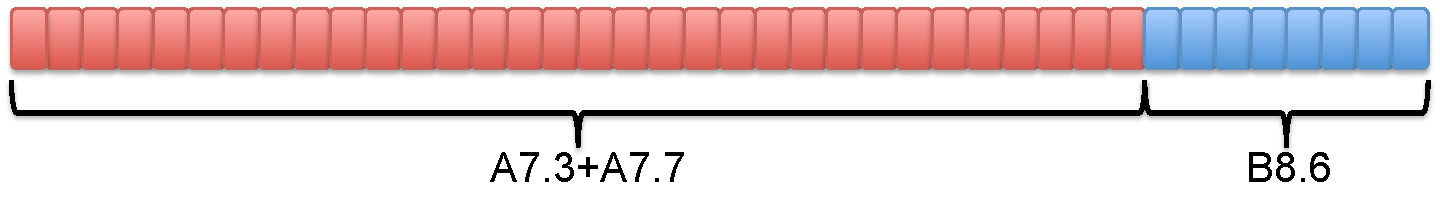
\includegraphics[scale=0.5]{figures/noto_cells.pdf}
\caption{\textbf{Notochord cells.}The primary notochord cell (blue) also known as the A-lineage are specified at the 64-cell stage. There are a total of 32 primary notochord cell that come from the A7.3 and A7.7 blastomere, and the intercalation of the cell happen in a semi-random stochastic manner.The secondary notochord cells (red) comes from the B8.6 blastomere and are specified at the 110-cell stage, one cell division after the primary notochord cells.}
\label{fig:noto_cells}
\end{figure}

Although a tailed larvae is typical of most ascidians, several species with in the Stolidobranchia order have individually undergone tail-loss, many of which fall in the Molgulidae \cite{berrill_studies_1931, jeffery_evolution_1999, huber_evolution_2000, maliska_molgula_2010}. The tail-less\textemdash anural\textemdash species develop in a similar manner and are indistinguishable from their tailed\textemdash urodele\textemdash counterparts up to late gastrulation \cite{berrill_studies_1931, swalla_interspecific_1990, jeffery_factors_1992}. Anural ascidians lack several urodele features including an intercalated and extended notochord, differentiated muscle cells and the otilith sensory organ. The absence of differentiated muscles cells and intercalated notochord are the cause for the lack of tail in these species \cite{miyamoto_formation_1985, swalla_interspecific_1990}. The development of several tail-less species have been studied. \textit{M. tectiformis} notochord cells do not divide again after the 10 precursor cells are formed and \textit{M. occulta} stops dividing after 20 cells \cite{jeffery_evolution_1999}. The same occurs in \textit{M. bleizi}, however after the 20 notochord cells are formed, the embryo attempts to make a tail but never completes the process \cite{swalla_novel_1993}. It has also been shown that chordate embryos without fully developed notochord and/or muscle cells do not fully elongate or fail completely to develop a tail \cite{jeffery_evolution_1999,takada_brachyury_2002,stemple_structure_2005}. 
Seeing that most ascidians have tailed larvae and that the tail can be restored through the use of interspecies hybrids, the lack of tail has been shown to be a loss of function. \textit{M. oculata} and \textit{M. occulta} both of the Roscovita clade have been shown to produce hybrids in lab conditions. Of the known \textit{Molgula} species \textit{M. occulta} and \textit{M. oculata} are the only two that can hybridize. Although \textit{M. occulta} and \textit{M. oculata} have been found to dwell in the same habitat, hybrids have not been found in nature and have only been produced in lab conditions. Fertilizing \textit{M. oculata} eggs with \textit{M. occulta} sperm in most cases produce embryos with fully formed tails. The reciprocal hybrid produces an embryo with 20 notochord cells like \textit{M. occulta}, however the notochord cells converge and extent like \textit{M. oculata} \cite{swalla_interspecific_1990}. The ascidian tail has been shown to form in the presence of notochord and the absence of muscles cells \cite{miyamoto_formation_1985} and the hybrid tail is not flaked by muscles as that of tail species \cite{swalla_novel_1993}. However, also it has been shown that embryos that develop urodele features are batch specific, and only in embryos that express the p58 which is associated with cytoskeleton are urodele features restored \cite{swalla_identification_1991,jeffery_factors_1992}. It has also been shown that in hybrid embryos in which urodele features were restored, the number of cells that express acetylcholinesterase (AChE) in a vestigial muscle cell lineage increased in comparison to hybrids lacking urodele features and \textit{M. occulta} \cite{jeffery_evolutionary_1991}. This along with evidence that with may have been, the ancestral notochord\textemdash the axochord\textemdash is muscle based \cite{lauri_development_2014}, shows strong evidence for the need of both notochord and muscles cells for the formation of the ascidian tail. 

\section{Brachyury has been shown to be the  }

\textit{Brachyury} a T-box transcription factor, has been identified to be essential for notochord development \cite{yasuo_conservation_1998}. The notochord induction is regulated by the \textit{FGF/MAPK/Ets} signaling cascade \cite{minokawa_binary_2001}. Where the A6.2 and A6.4 notochord/nerve cord precursors are induced by \textit{FGF9/16/20} at the 32-cell stage, just after the 7th cell cleavage \cite{satoh_ascidian_2001}. It was observed from isolation experiments that notochord/nerve cord precursors that loss \textit{FGF9/16/20} competence at the 32-cell stage assume the default nerve cord cell fate, the converse is true for presumptive nerve cord blastomeres that are introduce to \textit{FGF}, they forgo their default nerve cord fate and choose the notochord fate \cite{yasuo_conservation_1998,minokawa_binary_2001}. If \textit{FGF9/16/20} is not present at the 32 cell stage competence is lost, \textit{bra} is not induced and the notochord can no longer from \cite{nakatani_basic_1996,nakatani_duration_1999}. This is because \textit{MAPK} is not activated and the induction of \textit{bra} and repression of \textit{FoxB} are not carried out \cite{hashimoto_transcription_2011}. Without the repression of \textit{FoxB TF} the notochord cell fate is repressed through the repression of \textit{bra}. It has been observed in \textit{H. roretzi} that \textit{FoxB} represses the activation of \textit{bra} predominately through the binding of Fox BS1 (GCACTGA\textit{ACAAACA}TACATAG). \textit{FoxB} is activated by \textit{ZicN} and present in both nerve cord and notochords precursors, however is repressed by \textit{MAPK} in the notochord cell lineage at the 64-cell stage \cite{hashimoto_transcription_2011}. \textit{MAPK} is thought to be repressed by \textit{Ephin} which is one of the key differences between notochord and nerve cord determination. At this point \textit{bra} is expressed first weakly in the at the 64-cell stage in the notochord/nerve chord precursors \cite{yasuo_ascidian_1994} and unlike other chordates, in ascidians \textit{bra} is only expressed in the notochord cells \cite{yasuo_function_1993,corbo_characterization_1997,hotta_temporal_1999,takada_brachyury_2002}. Although \textit{bra} is necessary, its presence does not guarantee a tail. \textit{M. occulta} and \textit{M. tectiformis}, two tailless \textit{Molgula}, both express \textit{bra}. In both cases \textit{bra} expression stop earlier than that of \textit{M. oculata}, but produce different results. \textit{Bra} is expressed in the 10 precursor notochord cells in \textit{M. occulta}, another round of cell division occurs which does not in \textit{M. tectiformis}.  In these two species of \textit{Molgula} muscle actin became pseudo genes, however the mutation in the muscle actin genes are not the same \cite{swalla_novel_1993,jeffery_evolution_1999}. \textit{Manx} is another gene identified to be important for tell development in \textit{Molgula}, and is lowly expressed in \textit{M. occulta}, and has been shown to restore the hybrid tail \cite{swalla_requirement_1996, swalla_multigene_1999}. 
  
After cell specification, the notochord cells must converge, intercalate and extend. The Planar Cell Polarity (PCP) pathway is involved in cell movement during this process and mutations in \textit{prickle}\textemdash a known PCP gene\textemdash have shown to cause a shortened ascidian tail affecting both the mediolateral intercalation and the elongation of the ascidan tail \cite{jiang_ascidian_2005}. The \textit{pk} mutant \textit{aimless} produces a truncated tail, however the polarity of the nuclei are present, showing that prickle does not establish polarity with in the cell but polarity between cells, acting in a local manner and perhaps their is a global organizer \cite{jiang_ascidian_2005,kourakis_one-dimensional_2014}. However, even in the absence of the PCP pathway considerable convergence and elongation of the notochord was observed in Ciona, driven by a presumed boundary effects \cite{veeman_chongmague_2008}.

Many of the upstream genes and transcription factors that interact with \textit{bra} has been studied in fair detail, through known-outs, and cell isolation experiments. Not as much detail is known about the downstream genes regulated by \textit{bra}. On larger scale subtractive screening was done to identify genes downstream of \textit{bra}, 39 genes were initially found \cite{hotta_temporal_1999}. An attempt to characterize a number of these genes have been made, identifying functions such as extracellular matrix components (\textit{cadherin 8, entactin, fibronectin, laminin $alpha$1, $alpha$4, and $beta$1, and thrombospondin}, genes involved in cell shape and polarity (\textit{pk, trop, ERM, ACL}), axon guidance (\textit{netrin, semaphorin 3A}), amongst a host of other biological processes \cite{hotta_characterization_2000,hotta_brachyury-downstream_2007,kugler_evolutionary_2008}. 

\textit{Oikopleura} which are in the same subphyla\textemdash tunicates or urochordates\textemdash also develops in a typical chordate manner with a notochord and has a compact genome, however, in Larvacean there are 20 notochord cells \cite{seo_miniature_2001,denoeud_plasticity_2010}. \textit{Oikopleura} retains its tail during its adult life stage and at this point \textit{bra} is not expressed in the adult notochord, however, \textit{bra} is expressed in the same manner in the developing larval notochord as ascidians \cite{bassham_brachyury_2000,nishida_development_2008}. When comparing gene networks, \textit{Oikopleura} did not exhibit the same mechanism for tail development as \textit{Ciona}, of the 50 bra target genes previously identified cite only 26 of them had orthologs, almost 50\% of the genes were not present \cite{kugler_evolutionary_2011}. Of the genes that did show homology, expression ranged from notochord specific to tail including possible notochord, to tissues that were clearly not the notochord.


\section{Assembling and analyzing data}
One of the major advances in science in the past 20 years was the implementation of sequencing technologies. These technologies allowed us to examine problems in ways not previously possible. The first wave was Sanger sequencing in the 1986, but was not broadly used until 10 years later. Another technology, mircoarrays, which became popular starting in the mid '90s, allow us to look at a wide spectrum of genes and understand relative expression within a sample. Kobayashi et al. \cite{kobayashi_differential_2013} isolated and analyzed gene expression in notochord (A7.3+A7.7) and nerve cord (A7.4+A7.8) precursors using microarrays. This study was able to identify 106 genes expressed in the notochord precursor and 68 expressed in the nerve cord precursor at the 64-cell stage. Of these the genes, 36 notochord genes and 25 nerve chord genes were confirmed via Whole Mount In Situ Hybridization in the respective cells. This demonstrates the power of this technique, however, prior knowledge is needed. \textit{C. intestinalis} was sequenced using sanger sequencing, and is well assembled and most well annotated \cite{dehal_draft_2002}. In addition to long reads (Sanger) scaffolding was done using experimental data\cite{satou_improved_2008}. Sanger sequencing able to sequence whole genomes without the need of prior knowledge to identify novel genes but is costly and time consuming\cite{metzker_emerging_2005,liu_comparison_2012}. 

Sanger was the $1$\textsuperscript{st} generation of sequencing technologies, and currently both $2$\textsuperscript{nd} and $3$\textsuperscript{rd} generation are in use, with Roche 454, Ion Torrent, Illumina and PacBio are the most wide spread. These technologies are far easier to produce data and much less costly than sanger sequencing \cite{metzker_emerging_2005}. There are many trade-offs for each of the technologies, cost per MB, sequencing time, prep cost, error rate and sequencing bias; 454 and PacBio have longer reads than Illumina and Ion Torrent, 800 bp and 1+kbp, respectively. However, both Illumina and Ion Torrent's short reads are cheaper to generate, produce more reads and better for counting, in addition to PacBio having a high error rate \cite{glenn_field_2011}. Illumina and Ion Torrent have the best error rates and while Ion Torrent calls more more Single nucleotide polymorphisms, it also calls more false positives.  For this reason, amongst other Illumina is the most used because it is the most versatile and preforms the best in general \cite{quail_tale_2012}. This drop in price and produced many of the assembled genomes within the Tuncata phyla. Outside of this project there are eight tunicate genomes assembled; \textit{C. intestinalis}, \textit{C. savignyi}, \textit{Oikopleura dioica}, \textit{Botryllus schlosseri}, \textit{Halocynthia uranium}, \textit{H. foretzi}, \textit{Phallusia fumigata}, and \textit{P. mammilata}, but no \textit{Molgula} genomes. 

\chapter{Measuring the metrics}



\chapter{Another chapter}

\chapter{Conclusions}
The chordate body plans is fairly conserved throughout the phyla, with most developing into a tadpole larvae containing a hollow dorsal neural tube, and a postanal tail containing a notochord flanked by muscle cells. Molguilds are especially useful models because for studying the development of body plans because they have both tailed and tail-less species, two of which has the ability to produce interspecific hybrids. This allows us to examine the mechanisms of evolutionary divergent body plans at an allele-specific level. 

\section{Evaluating a lightweight transcriptome assembly pipeline on two closely related ascidian species}
Many non-model systems are now being sequenced with the drop in sequencing price. The methodology for assembly is not cut and dry, there are number step\textemdash quality trimming, filtering, choice of assembler and metrics to evaluate assembly. One of the standard is the N50, which has been designed for genomes and does not clearly translate to transcriptomes because of their fragmented nature, and the likelihood of chimeric contigs. We show that pre filtering quality trimmed assembly reads does not reduce the information content of the assembly. Many times assembly methods are chosen on the usability of software and the availability of resources. We have demonstrated that the Oases and Trinity assemblers returns similar results, suitable for downstream analysis. Our pipelines are available so we also provide methodology to be used by future researchers. 

\subsection{Contributions}
The experimental design for the RNA sequence analysis was decided by C. Titus Brown (CTB) and Billie J. Swalla (BJS). The fertilization and collection of RNA samples were done by BJS and myself. Library preparation for Illumina sequencing was done by Kanchan Pavangadkar. All downstream analysis was done by myself. The idea for evaluating de novo assembly pipeline came about through conversations with CTB, as well as methods for evaluation the transcriptome assemblies. Writing was done by me with edits from BJS and CTB.

\section{Genome assembly and characterization}
\subsection{Contributions}
The experimental design for the DNA sequencing was decided by CTB, BJS, and Lionel Christiaen (LC). Embryonic samples were collected by BJS, LC, Alberto Stolfi (AS), Claudia Racioppi (CR) and myself. Genome assembly was conducted by me. Ideas for examining divegand were developed by AS, orthologous sequences were identified through the use of RBH blast and done so by me because the sequences were not yet search about on the Aniseed database. The \textit{Hox} analysis was done by me and was conduced because of a question from David Arnosti. Writing was done by AS, myself with edits from BJS, CTB, CR, and LC.

\section{Differential expression analysis of tail loss in an invertebrate chordate}
Studying closely related organisms gives us insight into the underlying evolutionary mechanisms of divergence and underlying development. Indirect and direct developing sea urchins have been studied showing that change in axis and cell fate leads to divergent larval body plans that exhibits similar adults \cite{}. In contrast, ascidians retain their typical cell division and invariant cell fate. This is evident in both direct and indirect tail-less ascidians \cite{}. 
\subsection{Contributions}
The experimental design is the same for the "Evaluating a lightweight transcriptome assembly pipeline on two closely related ascidian species" chapter (3). Transcript models were assembled by me. Read mapping for differential expression analysis was conducted by me, and the analysis of hybrid expression counts were the idea of CTB. The differential expression analysis was conducted by me, including the idea to focus on the overlapping upregulated gene in \textit{M. oculata} and the interspecific hybrid. Annotation of the overlapping upregulated genes was done by AS, Anna Di Gregorio and myself. Writing was done by me with edits from AS, CR, and CTB.
  
Next generation sequencing is a great way to study non-model species. A broad swath of information can be gained from both RNA and DNA sequencing. This technology has allowed us to analyzed two closely related invertebrate chordates that also hybridize. This study has given us insight into the mechanisms behind tail-loss and development. Gene loss has occurred but other factors appear to be involved in tail-loss because expression from the tailed species appears to recover the loss features. 


%%%%%%%    APPENDICES    %%%%%%%%%%
%% If you wish to include one appendix, remove the "%" from the 
%% following two lines.
\renewcommand{\appname}{APPENDIX}
\appendix
ascidian
notochord
tunicate
NGS
rna-seq
de novo assembly
mapped based assembly
urdele
anural
M. occulta
M. oculata
M. occidentalis
C. intestinalis

%% To include several appendices, remove the only the "%"
%% in front of "\appendix".

%% In either cast to start your first appendix, which will be labeled
%% as Appendix A, just type \chapter{<appendix 1 name>}
%% and enter the text of the appendix as you would a chapter.

%%%%%%% A NOTE ABOUT APPENDICES %%%%%%%%%
%% Some appendices may be single spaced such as survey examples or letters.
%% Contact the Graduate School for details.
%% To single space an appendix first remove the % from 
%% the following two lines. 
% \end{doublespace}
% \chapter{<appendix  name>}
%% After entering the appendix remove the % from 
%% the following line
% \begin{doublespace}
%% Any text entered now will be double spaced.
\end{doublespace}

%%Bibliography 

%% A bibliography is required. By default it is called, "Bibliography"
%% You may use �Literature Cited�, �Works Cited� or �References� 
%% instead of �Bibliography� if that is the convention in your discipline. 
%% To do so, place your choice in the  empty argument 
%% of the following command and remove the "%".
\renewcommand{\bibname}{BIBLIOGRAPHY}
%% The bibliography may be made using BibTeX.
%% If it's made from scratch,
%% remove the "%" in front of "\begin{thebibliography}{???}"
%% replacing the ??? with the appropriate entry and 
%% remove the "%" in front of "\end{thebibliography}"
% \begin{thebibliography}{???}
%%  Enter the bibliography here.
% \end{thebibliography}

\bibliographystyle{abbrv}
\bibliography{MyLibrary}

\end{document}
